\documentclass[11pt]{beamer}
\usepackage[utf8]{inputenc}
\usepackage[T1]{fontenc}
\usepackage{lmodern}
\usepackage[french]{babel}
\usetheme{Antibes}
\usepackage{subfig}
\usepackage{algorithm}
\usepackage{algorithmic}
%%% Packages additionnels
\usepackage{verbatim}
\usepackage{bbm}
\usepackage{stmaryrd}
\usepackage[numbered,framed]{matlab-prettifier}
\usepackage{listings}

\renewcommand{\algorithmicrequire}{\textbf{Entrée(s) :}}
\renewcommand{\algorithmicreturn}{\textbf{retourner}}
\renewcommand{\algorithmicensure}{\textbf{Initialisation ;}}
\renewcommand{\algorithmicwhile}{\textbf{Tant que}}
\renewcommand{\algorithmicdo}{\textbf{Initialisation}}
\renewcommand{\algorithmicendwhile}{\textbf{fin du Tant que ;}}
\renewcommand{\algorithmicend}{\textbf{fin}}
\renewcommand{\algorithmicif}{\textbf{si}}
\renewcommand{\algorithmicendif}{\textbf{fin du si}}
\renewcommand{\algorithmicelse}{\textbf{sinon}}
\renewcommand{\algorithmicelsif}{\textbf{fin du sinon}}
\renewcommand{\algorithmicthen}{\textbf{alors}}
\renewcommand{\algorithmicthen}{\textbf{Étape E}}
\renewcommand{\algorithmicthen}{\textbf{Étape M}}
\renewcommand{\algorithmicfor}{\textbf{pour}}
\renewcommand{\algorithmicforall}{\textbf{pour tout}}
\renewcommand{\algorithmicto}{\textbf{à}}
\renewcommand{\algorithmicendfor}{\textbf{fin du pour}}
\renewcommand{\algorithmicdo}{\textbf{faire}}
\renewcommand{\algorithmicloop}{\textbf{boucler}}
\renewcommand{\algorithmicendloop}{\textbf{fin de la boucle}}
\renewcommand{\algorithmicrepeat}{\textbf{répéter}}
\renewcommand{\algorithmicuntil}{\textbf{jusqu’à}}

\setbeamertemplate{blocks}[rounded][shadow=true]
\makeatother
\setbeamertemplate{footline}
{
	\leavevmode%
	\hbox{%
		\begin{beamercolorbox}[wd=.33\paperwidth,ht=2.25ex,dp=1ex,center]{author in head/foot}%
			\usebeamerfont{author in head/foot}\insertshortauthor
		\end{beamercolorbox}%
		\begin{beamercolorbox}[wd=.33\paperwidth,ht=2.25ex,dp=1ex,center]{title in head/foot}%
			\usebeamerfont{title in head/foot}\insertshorttitle
		\end{beamercolorbox}%
		\begin{beamercolorbox}[wd=.33\paperwidth,ht=2.25ex,dp=1ex,center]{date in head/foot}%
			\usebeamerfont{date in head/foot}\insertshortdate\hspace*{3em}
			\insertframenumber{} / \inserttotalframenumber\hspace*{1ex}
	\end{beamercolorbox}}%
	\vskip0pt%
}
\makeatletter
\setbeamertemplate{itemize item}[ball]
\setbeamertemplate{itemize subitem}[triangle]
\setbeamertemplate{itemize subsubitem}[circle]



\AtBeginSection[]{\begin{frame} \tableofcontents[currentsection] \end{frame}}


\begin{document}
	\author{CÔME, SENE}
	\title[Projet UE HAX916X]{Projet Crowdsourcing}
	\subtitle{}
	\logo{
		\begin{minipage}[c]{1.15\linewidth}
			
\includegraphics[height=0.6cm]{logo.png} \hspace{0.65truecm}\hfill 
			
\includegraphics[height=0.6cm]{imag_logo.png}
			\hspace{0.65truecm}\hfill 
			
\includegraphics[height=0.65cm]{images/ssd.png}
		\end{minipage}
	}
	\institute[Université de Montpellier]{Présentation de projet de Master 2}
	\date{3 Janvier 2023}
	%\subject{}
	%\setbeamercovered{transparent}
	\setbeamertemplate{navigation symbols}{}
	%	\begin{frame}[plain]
		%		\maketitle
		%	\end{frame}
	\frame{\titlepage}
	%	\begin{frame}
		%		\frametitle{}
		%	\end{frame}
	
	%%%%%%%%%%%%%%%%%%%%%%%
	\begin{frame}{Introduction}
		\begin{block}{Contexte}
			\begin{itemize}
				\item Utilisation de l'Algorithme EM pour connaitre le vrai label d'une image donnée ou déterminer la véritable pathologie d'un patient.
				\item Type de données : 60000 images $32\times32$ séparées en 10 classes
				\item Problématique : La labélisation d'une image donnée ou le diagnostic d'un patient.
				\item Approche classique : affichage de la matrice de confusion à l'aide de l'algorithme EM.
			\end{itemize}
		\end{block}
	\end{frame}
	
%	\begin{frame}
%		\begin{block}{}
%			\begin{figure}[H]
%				\centering
%				\includegraphics[scale=0.7]{images/data_wine.png}
%				\caption{Exemple de données catégorielles ordonnées}
%			\end{figure}
%		\end{block}
%	\end{frame}
	
	
	\section{Notations}
	\begin{frame}{Notations}
		\begin{block}{Notations}
			On note $\forall i \in \{1, 2, \dots,I\}$, $\forall j, l \in \{1, 2, \dots,J\}$, $\forall k \in \{1, 2, \dots,K\}$ : \\
			\begin{itemize}
				\item $\pi_{lj}^k$ : la probabilité que le médecin k donne la réponse j sachant que la vraie réponse est l.
				\item $T_{ij}$ : une variable de réponse associée au patient i définie par $T_{iq} = 1$  si q est la vraie réponse et $T_{iq} = 0$ si $j \neq q$.
				\item $p_j$ : la prévalence de la classe j ou la fréquence empirique.
				
			\end{itemize} 
			
		\end{block}
	\end{frame}
	
	\section{Estimation de la vraisemblance}
	\begin{frame}{Cas 1}
		\begin{block}{1 medecin 1 patient}	
			
			Soit $X$ à valeur dans $\{1, 2, \dots ,M\}$, une variable aléatoire indiquant la maladie du patient.
			
			Soit $Y$ à valeur dans $\{1, 2, \dots ,J\}$, une variable aléatoire correspondant à la maladie du patient indiquée par le médecin.																												
			
			\[Y | X=x \sim Multinomiale \left[(\pi_{xl}^Y)_{l}, n\right], avec\hspace{2mm}l \in \{1, 2, \dots,J\} .\]
		\end{block}
	\end{frame}
	
	
	\begin{frame}{Cas 1}
		\begin{block}{1 médecin 1 patient}	
			
			Sa fonction de masse est donnée par : \[\mathbb{P}\left(n_{i1}^k, \dots, n_{iJ}^k\right) = \frac{\left[\sum_{j=1}^{J} n_{ij}^k\right]!}{\prod_{j=1}^{J} n_{ij}^k !} \prod_{j=1}^{J} \left(\pi_{lj}^k\right)^{{n_{ij}}^{k}} \propto \prod_{j=1}^{J} \left(\pi_{lj}^k\right)^{{n_{ij}}^{k}}.\]
			Ainsi la vraisemblance est : \[\propto \prod_{j=1}^{J} \left(\pi_{lj}^k\right)^{{n_{ij}}^{k}}\]
			
		\end{block}
	\end{frame}
	
	\begin{frame}{Cas 2}
		\begin{block}{K medecins et I patients}
			Soit $X$ = $(X_1, \dots, X_I)$ le vecteur aléatoire indiquant la maladie des I patients.\\
			Soit $Y$ = $(Y_1, \dots, Y_K)$ le vecteur aléatoire indiquant la maladie des K patients.\\
			Si le médecin répond une fois à la question du patient, on a :
			\[Y_{i}^k | X_i=x_i \sim Multinomiale \left[(\pi_{x_ij}^k), 1\right],\]\\
			$avec\hspace{2mm}j \in \{1, 2, \dots,J\}\hspace{2mm} et\hspace{2mm} i \in \{1, 2, \dots,I\}$
			
		\end{block}
	\end{frame}	
	
	\begin{frame}{Cas 2}
		\begin{block}{K medecins et I patients}
			Étant donné que les $(Y_{i}^k)$ sont indépendants $ \forall\hspace{2mm}k \in \{1, 2, \dots,K\}\hspace{2mm} et\hspace{2mm} i \in \{1, 2, \dots,I\}$, Donc : \[\mathbb{P}\left(n_{i1}^k, \dots, n_{iJ}^k\right) = \frac{\left[\sum_{j=1}^{J} n_{ij}^k\right]!}{\prod_{j=1}^{J} n_{ij}^k !} \prod_{j=1}^{J} \left(\pi_{x_ij}^k\right)^{{n_{ij}}^{k}} \propto \prod_{k=1}^{K} \prod_{j=1}^{J} \left(\pi_{x_ij}^k\right)^{{n_{ij}}^{k}}.\]
			Par conséquent la vraisemblance est : \[\propto \prod_{k=1}^{K} \prod_{j=1}^{J} \left(\pi_{x_ij}^k\right)^{{n_{ij}}^{k}}\]
			
		\end{block}
	\end{frame}	
	
	\begin{frame}{Cas 2}
		\begin{block}{Toutes les données}
			Si on se base sur toutes les données c'est-à-dire les réponses de tous les médecins et les questions de tous les patients, on a :
			\[\mathbb{P} \left((\cap \cap Y_{i}^k) | \cap(X_i=x_i) \right) \mathbb{P}\left(\cap (X_i = x_i)\right) \] = \[\mathbb{P} \left((\cap \cap Y_{i}^k) \cap \left(\cap(X_i=x_i)\right)  \right).\]
			Par indépendance des $(Y_{i}^k)$ et $(X_i)$, 
			
		\end{block}
	\end{frame}	
	
	\begin{frame}{Cas 2}
		\begin{block}{Toutes les données}
			\scriptsize
			\begin{align*}
				\mathbb{P} \left((\cap \cap Y_{i}^k) \cap \left(\cap(X_i=x_i)\right)  \right) &= \prod_{i=1}^{I} \mathbb{P} \left(\cap Y_{i}^k | \cap (X_i=x_i)\right) \mathbb{P}(X_i = x_i)\\
				&= \prod_{i=1}^{I}\left(\mathbb{P}(X_i = x_i) \prod_{k=1}^{K}\mathbb{P} \left( Y_{i}^k | \cap(X_i=x_i) \right)\right) \\
				&= \prod_{i=1}^{I}\left(p_{x_i} \prod_{k=1}^{K}\mathbb{P} \left( Y_{i}^k | (X_i=x_i) \right)\right)
			\end{align*}
			
		\end{block}
	\end{frame}	
	
	\begin{frame}{Cas 2}
		\begin{block}{Toutes les données}
			D'où \[\mathbb{P} \left((\cap \cap Y_{i}^k) \cap \left(\cap(X_i=x_i)\right)  \right) \propto \prod_{i=1}^{I}\prod_{l=1}^{J}\left[p_{x_i} \prod_{k=1}^{K} \prod_{j=1}^{J} \left(\pi_{ij}^k\right)^{{n_{ij}}^{k}}\right]^{T_{ij}}.\]
			Par conséquent la vraisemblance de toutes les données est :
			\[\propto \prod_{i=1}^{I}\prod_{l=1}^{J}\left[p_{x_i} \prod_{k=1}^{K} \prod_{j=1}^{J} \left(\pi_{ij}^k\right)^{{n_{ij}}^{k}}\right]^{T_{ij}}\]	
			
		\end{block}
	\end{frame}	
	
	\section{Estimation du maximum de vraisemblance}
	\begin{frame}{Les estimateurs}
		\begin{block}{Expressions}
			Si on suppose que les $T_{ij}$ sont connus et que en pratique nous avons les ${{n_{ij}}^{k}}$, on a les estimateurs du maximum de vraisemblance suivants :
			\[\hat{\pi}_{jl}^k = \frac{\sum_{i=1}^{I} T_{ij} {n_{il}}^{k}}{\sum_{l=1}^{J} \sum_{i=1}^{I}  T_{ij} {n_{il}}^{k}}.\]\\
			\[\hat{p}_j = \frac{\sum_{i=1}^{I} T_{ij}}{I}.\]
		\end{block}
	\end{frame}

	\section{Le jeu de données}
	\begin{frame}{cifar10h}
		Base de données composée de 10 classes d'images:
		\begin{itemize}
			\item classe 0: airplane \\
			\item classe 1: automobile \\
			\item classe 2: bird \\
			\item classe 3: cat \\
			\item classe 4 deer \\
			\item classe 5: dog \\
			\item classe 6: frog \\
			\item classe 7: horse \\
			\item classe 8: ship \\
			\item classe 9: truck
		\end{itemize}
	\end{frame}
	
	\begin{frame}{cifar10h}
		\begin{figure}[H]
			\centering
			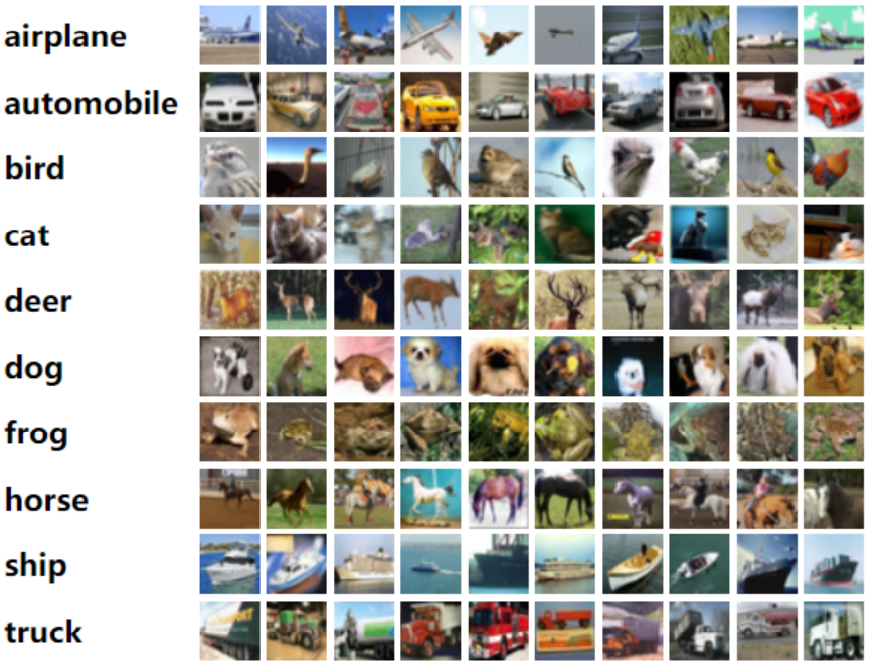
\includegraphics[scale=0.45]{images/imagecifar10.png}
			\caption{Un extrait de la base de données}
		\end{figure}
	\end{frame}
	
	\section{Fonctions utiles pour réaliser les expériences numériques}
	\begin{frame}{La fonction $CreateSubDf$}
		\scriptsize
		\begin{block}{Son objectif}
			Créer un sous dataframe dans lequel seront stockées uniquement les données utiles:
	    \end{block}
    	\begin{block}{Ses arguments}
    		\begin{itemize}
    			\item \textit{\textbf{df:}} le dataframe des données (Il s'agit du dataframe d'origine) \\
    			\item \textbf{\textit{an\_id:}}  entier (compris entre 0 et 2570) désignant l'identifiant de l'annotateur
    		\end{itemize}
    	\end{block}
    \begin{block}{Ce qu'elle retourne}
    	Un sous dataframe composé de deux colonnes:
    	\begin{itemize}
    		\item \textbf{\textit{La colonne 1:}} contient les labels choisis par un annotateur spécifique
    		\item \textbf{\textit{La colonne 2:}} contient les vrais labels associés aux images
    	\end{itemize} 
    \end{block}
	\end{frame}

	\begin{frame}{La fonction $custom\_confusion\_matrix$}
		\small
		\begin{block}{Son objectif}
			Améliorer l'esthétique de la représentation graphique de la matrice de confusion
		\end{block}
		\begin{block}{Ses arguments}
			\begin{itemize}
			\item \textbf{\textit{cm:}} un 2D numpy array jouant le rôle de la matrice de confusion \\
			\item \textbf{\textit{classes:}} la liste stockant les noms de chaque classe \\
			\item \textbf{\textit{normalize:}} (Booléen): si True la matrice sera normalisée, et si False elle ne le sera pas \\
			\item \textbf{\textit{title:}} le titre du graphique \\
			\item \textbf{\textit{cmap:}} la palette de couleur du graphique
			\end{itemize}
		\end{block}
	\end{frame}

	\begin{frame}{La fonction $plot\_confusion\_matrix$}
		\scriptsize
		\begin{block}{Son objectif}
			Calculer la matrice de confusion et afficher sa représentation graphique
		\end{block}
		\begin{block}{Ses arguments}
			\begin{itemize}
				\item \textbf{\textit{y\_true:}} un numpy array dans lequel sont stockés les vrais labels \\
				\item \textbf{\textit{y\_predict:}} un numpy array dans lequel sont stockés les labels choisis par l'annotateur \\
				\item \textbf{\textit{normalize(Booléen):}} si True la matrice sera normalisée, et si False elle ne le sera pas \\
				\item  \textbf{\textit{class\_names:}} la liste stockant les noms de chaque classe \\
			\end{itemize}
		\end{block}
		\begin{block}{Ce qu'elle retourne}
			retourne le graphique de la matrice de confusion
		\end{block}
	\end{frame}
	
	\begin{frame}{La fonction $DawidSkeneIID$}
		\begin{block}{Son objectif}
			Permet d'initialiser le modèle de David Skene
		\end{block}
		\begin{block}{Ses arguments}
			\begin{itemize}
				\item \textbf{\textit{ydims:}} un couple sous la forme (nombre de classes, nombre d'annotateurs) \\
				\item \textbf{\textit{max\_iter:}} Le nombre d'iterations souhaité de l'algorithme EM \\
				\item  \textbf{\textit{predict\_tol:}} un seuil de tolérance pour la prédiction
			\end{itemize}
		\end{block}
		\begin{block}{Ce qu'elle retourne}
			retourne le graphique de la matrice de confusion
		\end{block}
	\end{frame}

	\begin{frame}{La fonction $fit$}
		\begin{block}{Son objectif}
			Permet d'alimenter le modèle
		\end{block}
		\begin{block}{Ses arguments}
			\begin{itemize}
				\item \textbf{\textit{U:}} les données de dim = (N,K) avec N lignes et K annotateurs (dans notre cas k = 1) \\
				\item \textbf{\textit{priors:}} les probabilités du prior pour $\pi_z$ et $\psi_{u,z}^k = p\big(u_k = u | Z = z\big)$ \\
				\item \textbf{\textit{starts:}} tuple contenant les matrices ($\pi$ et $\psi$) des paramètres initiaux de l'algorithme EM
			\end{itemize}
		\end{block}
	\end{frame}
	\begin{frame}{La fonction $ plot\_cm\_d$}
		\scriptsize
		\begin{block}{Son objectif}
			 afficher la représentation graphique de la matrice de confusion
		\end{block}
		\begin{block}{Ses arguments}
			\begin{itemize}
				\item \textbf{\textit{U:}} les données de dim = (N,K) avec N lignes et K annotateur (dans notre cas k = 1) \\
				\item \textbf{\textit{priors:}} les probabilités du prior pour $\pi_z$ et $\psi_{u,z}^k = p\big(u_k = u | Z = z\big)$ \\
				\item \textbf{\textit{starts:}} tuple contenant les matrices ($\pi$ et $\psi$) des paramètres initiaux de l'algorithme EM
			\end{itemize}
		\end{block}
		\begin{block}{Ce qu'elle retourne}
			le graphique de la matrice de confusion estimée à l'aide de l'algorithme EM
		\end{block}
	\end{frame}

	\section{Expériences numériques}
	\begin{frame}{Expériences numériques}
		\begin{figure}[htp] 
			\centering
			\subfloat[Matrice de confusion associée aux labels prédits par un annotateur]{%
				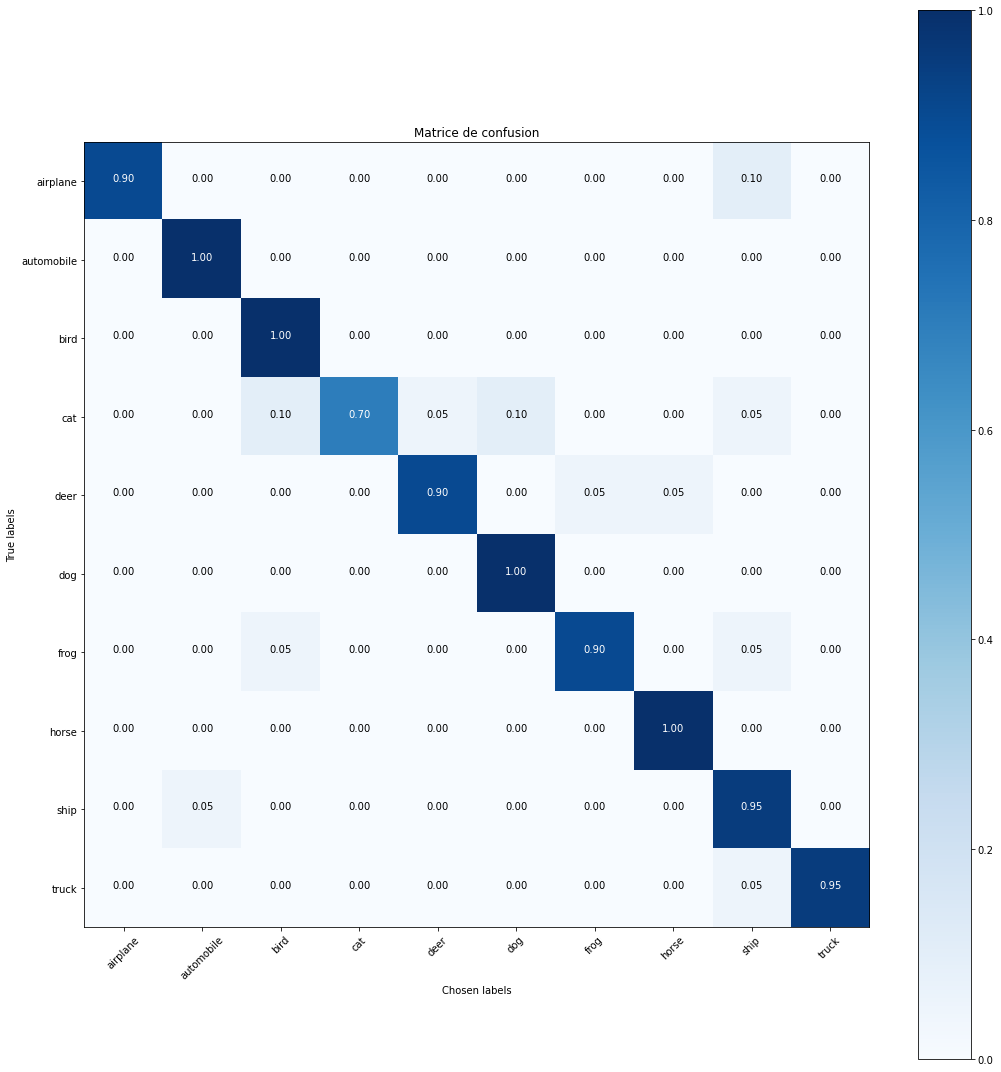
\includegraphics[scale=0.12]{images/cm.png}%
			}%
			\hfill%
			\subfloat[Matrice de confusion estimée à partir de l'algorithme EM]{%
				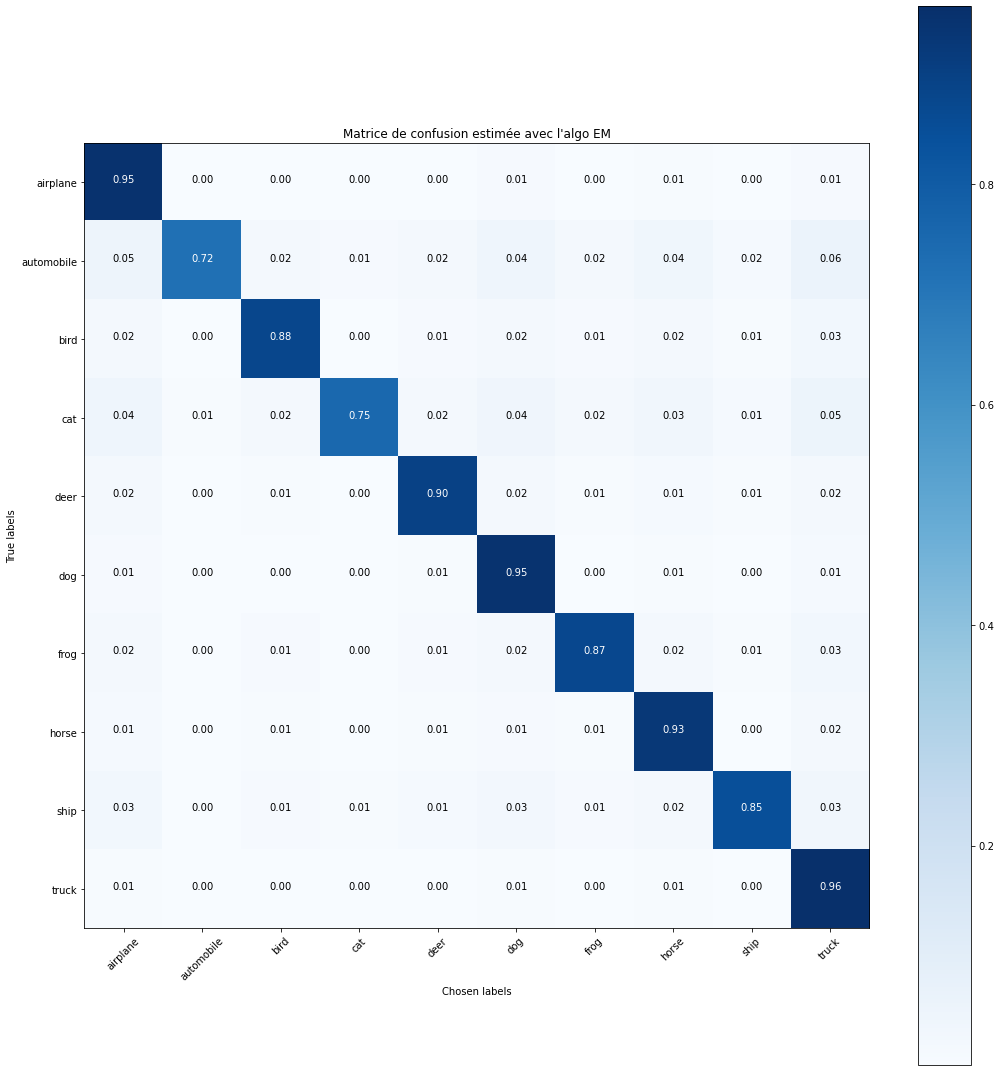
\includegraphics[scale=0.12]{images/cmEM.png}%
			}%
		\end{figure}
	\end{frame}

	\section{Conclusion}
	
	\begin{frame}{Conclusion}
		
		\begin{block}{Conclusion}
			D'après nos expériences numériques, nous constatons que :
			\begin{itemize}
				\item l'algorithme EM prédit bien nos images c'est-à-dire qu'il fait une bonne labélisation. En revanche, sa matrice de confusion n'est pas forcément meilleure que celle des annotateurs. 
				\item Cependant, malgré que la matrice de confusion des annotateurs ne montre pas beaucoup d'erreurs (presque diagonale), elle reste tout de même proche à celle de l'algorithme EM en terme de prédiction.
			\end{itemize}
			
		\end{block}
	\end{frame}
	


\end{document}
